\documentclass[f,master,twoside,binding,palatino]{AIGpaper}
% Please read the README.md file for additional information on the parameters and overall usage of AIGpaper

\usepackage{graphicx}					    % enhanced support for graphics
\usepackage{tabularx}				      	% more flexible tabular
\usepackage{amsfonts}					    % math fonts
\usepackage{amssymb}					    % math symbols
\usepackage{amsmath}					    % overall enhancements to math environment

% optional packages
\usepackage{tikz}                           % creating graphs and other structures
\usetikzlibrary{arrows,positioning}
\tikzset{
    %Define standard arrow tip
    >=stealth',
    %Define style for argument
    args/.style={circle, minimum size=0.9cm,draw=black, thick,fill=white},
}


% === set information ===
\author{Erika Mustermann}

\title{Die Verbreitung des Begriffes \glqq{}Mustermann\grqq{} im Zusammenhang mit Beispieltexten}

\degreecourse{Informatik}

\firstreviewer{Prof.\ Dr.\ Matthias Thimm}
\firstreviewerinfo{Artificial Intelligence Group}

\advisor{Max Mustermann}
\advisorinfo{Artificial Intelligence Group}

\englishabstract{%
Lorem ipsum dolor sit amet, consetetur sadipscing elitr, sed diam nonumy eirmod tempor invidunt ut labore et dolore magna aliquyam erat, sed diam voluptua. At vero eos et accusam et justo duo dolores et ea rebum. Stet clita kasd gubergren, no sea takimata sanctus est Lorem ipsum dolor sit amet. Lorem ipsum dolor sit amet, consetetur sadipscing elitr, sed diam nonumy eirmod tempor invidunt ut labore et dolore magna aliquyam erat, sed diam voluptua.
}
\germanabstract{%
Lorem ipsum dolor sit amet, consetetur sadipscing elitr, sed diam nonumy eirmod tempor invidunt ut labore et dolore magna aliquyam erat, sed diam voluptua. At vero eos et accusam et justo duo dolores et ea rebum. Stet clita kasd gubergren, no sea takimata sanctus est Lorem ipsum dolor sit amet. Lorem ipsum dolor sit amet, consetetur sadipscing elitr, sed diam nonumy eirmod tempor invidunt ut labore et dolore magna aliquyam erat, sed diam voluptua.
}

\begin{document}
\pagenumbering{roman}
\maketitle%prints the cover page  an empty page if two-sided print

% optional: change document language from ngerman to english
%\selectlanguage{english}

% disable tableofcontents and cleardoublepage for proposals
\tableofcontents%
\cleardoublepage%

% list of figures
% \listoffigures
% \varclearpage

\pagenumbering{arabic}


% ========== beginning of the actual text section ===========

\section{Lorem Ipsum}
Lorem ipsum dolor sit amet, consetetur sadipscing elitr, sed diam nonumy eirmod tempor invidunt ut labore et dolore magna aliquyam erat, sed diam voluptua. At vero eos et accusam et justo duo dolores et ea rebum. Stet clita kasd gubergren, no sea takimata sanctus est Lorem ipsum dolor sit amet. Lorem ipsum dolor sit amet, consetetur sadipscing elitr, sed diam nonumy eirmod tempor invidunt ut labore et dolore magna aliquyam erat, sed diam voluptua.\\
At vero eos et accusam et justo duo dolores et ea rebum. Stet clita kasd gubergren, no sea takimata sanctus est Lorem ipsum dolor sit amet.


\section{Example Figures and Tables}

Figure \ref{fig:af} shows an example of an abstract argumentation framework \cite{dung1995acceptability}.

\begin{figure}[ht]
    \centering
    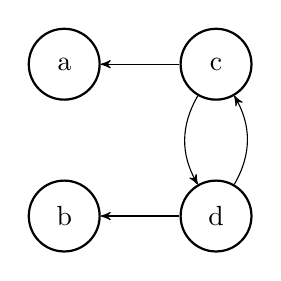
\begin{tikzpicture}[node distance=1cm]
    	\node[args](args1){a};
    	\node[args, below=of args1](args2){b};
    	\node[args, right=of args1](args3){c};
    	\node[args, right=of args2](args4){d};
    
        \path(args3) edge [->] (args1);
        \path(args3) edge [->, bend right] (args4);
        \path(args4) edge [->, bend right] (args3);
    	\path(args4) edge [->] (args2);
    	
    \end{tikzpicture}
    \caption{An abstract argumentation framework.}
    \label{fig:af}
\end{figure}

\begin{table*}[h]
\begin{center}
\begin{tabular}{lll}
\hline
1&2&3\\
4&5&6\\
\hline
\end{tabular}
\end{center}
\caption{Table caption.} 
\label{tab:t1}
\end{table*}



\subsection{Encoding Test}
Städte, Länder, Flüsse


% References
\addreferences

\end{document}
